\subsection{Example: A Picture Language}
\label{Section 2.2.4}

\begin{figure}[tb]
	\centering
	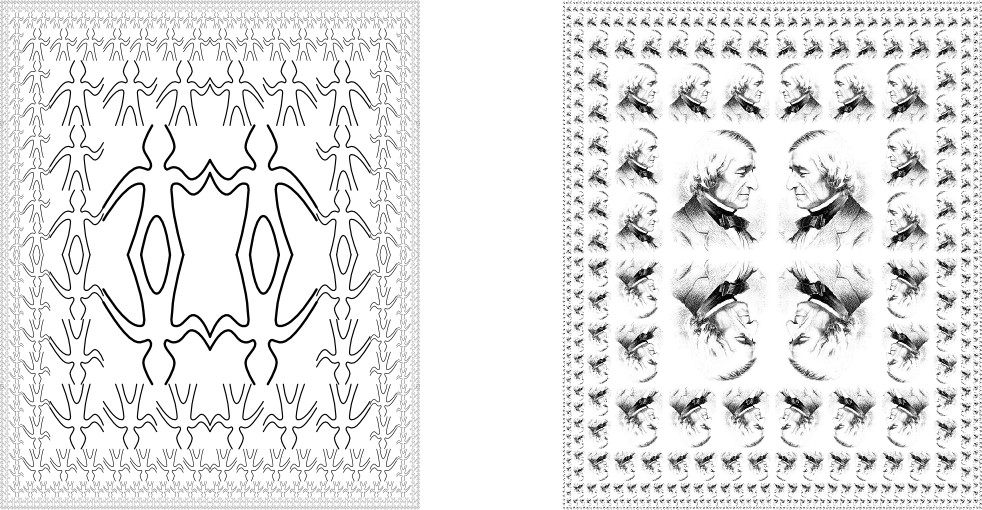
\includegraphics[width=111mm]{fig/chap2/Fig2.9-bigger.png}
	\caption{
		Designs generated with the picture language.
	}
	\label{Figure 2.9}
\end{figure}

This section presents a simple language for drawing pictures that illustrates the power of data abstraction and closure, and also exploits higher-order procedures in an essential way.
The language is designed to make it easy to experiment with patterns such as the ones in \cref{Figure 2.9}, which are composed of repeated elements that are shifted and scaled.%
\footnote{
	The picture language is based on the language Peter Henderson created to construct images like M.~C.~Escher’s “Square Limit” woodcut (see \cref{Henderson 1982}).
	The woodcut incorporates a repeated scaled pattern, similar to the arrangements drawn using the \code{square-limit} procedure in this section.
}
In this language, the data objects being combined are represented as procedures rather than as list structure.
Just as \code{cons}, which satisfies the closure property, allowed us to easily build arbitrarily complicated list structure, the operations in this language, which also satisfy the closure property, allow us to easily build arbitrarily complicated patterns.



\subsubsection*{The picture language}

When we began our study of programming in \cref{Section 1.1}, we emphasized the importance of describing a language by focusing on the language’s primitives, its means of combination, and its means of abstraction.
We’ll follow that framework here.

\begin{figure}[tb]
	\centering
	\includesvg[width=50mm]{fig/chap2/Fig2.10.svg}
	\caption{
		Images produced by the \code{wave} painter, with respect to four different frames.
		The frames, shown with dotted lines, are not part of the images.
	}
	\label{Figure 2.10}
\end{figure}

Part of the elegance of this picture language is that there is only one kind of element, called a \newterm{painter}.
A painter draws an image that is shifted and scaled to fit within a designated parallelogram-shaped frame.
For example, there’s a primitive painter we’ll call \code{wave} that makes a crude line drawing, as shown in \cref{Figure 2.10}.
The actual shape of the drawing depends on the frame---all four images in \cref{Figure 2.10} are produced by the same \code{wave} painter, but with respect to four different frames.
Painters can be more elaborate than this:
The primitive painter called \code{rogers} paints a picture of \acronym{MIT}’s founder, William Barton Rogers, as shown in \cref{Figure 2.11}.%
\footnote{
	William Barton Rogers (1804--1882) was the founder and first president of \acronym{MIT}.
	A geologist and talented teacher, he taught at William and Mary College and at the University of Virginia.
	In 1859 he moved to Boston, where he had more time for research, worked on a plan for establishing a “polytechnic institute,” and served as Massachusetts’s first State Inspector of Gas Meters.

	When \acronym{MIT} was established in 1861, Rogers was elected its first president.
	Rogers espoused an ideal of “useful learning” that was different from the university education of the time, with its overemphasis on the classics, which, as he wrote, “stand in the way of the broader, higher and more practical instruction and discipline of the natural and social sciences.”
	This education was likewise to be different from narrow trade-school education.
	In Rogers’s words:

	\begin{quote}
		The world-enforced distinction between the practical and the scientific worker
		is utterly futile, and the whole experience of modern times has demonstrated
		its utter worthlessness.
	\end{quote}

	Rogers served as president of \acronym{MIT} until 1870, when he resigned due to ill health.
	In 1878 the second president of \acronym{MIT}, John Runkle, resigned under the pressure of a financial crisis brought on by the Panic of 1873 and strain of fighting off attempts by Harvard to take over \acronym{MIT}.
	Rogers returned to hold the office of president until 1881.

	Rogers collapsed and died while addressing \acronym{MIT}’s graduating class at the commencement exercises of 1882.
	Runkle quoted Rogers’s last words in a memorial address delivered that same year:

	\begin{quote}
		“As I stand here today and see what the Institute is, … I call to mind the beginnings of science.
		I remember one hundred and fifty years ago Stephen Hales published a pamphlet on the subject of illuminating gas, in which he stated that his researches had demonstrated that 128 grains of bituminous coal---”

		“Bituminous coal,” these were his last words on earth.
		Here he bent forward, as if consulting some notes on the table before him, then slowly regaining an erect position, threw up his hands, and was translated from the scene of his earthly labors and triumphs to “the tomorrow of death,” where the mysteries of life are solved, and the disembodied spirit finds unending satisfaction in contemplating the new and still unfathomable mysteries of the infinite future.
	\end{quote}

	In the words of Francis A. Walker (\acronym{MIT}’s third president):

	\begin{quote}
		All his life he had borne himself most faithfully and heroically, and he died as so good a knight would surely have wished, in harness, at his post, and in the very part and act of public duty.
	\end{quote}
}
The four images in \cref{Figure 2.11} are drawn with respect to the same four frames as the \code{wave} images in \cref{Figure 2.10}.

\begin{figure}[tb]
	\centering
	\includesvg[width=48mm]{fig/chap2/Fig2.11.svg}
	\caption{
		Images of William Barton Rogers, founder and first president of \acronym{MIT}, painted with respect to the same four frames as in \cref{Figure 2.10} (original image from Wikimedia Commons).
	}
	\label{Figure 2.11}
\end{figure}

To combine images, we use various operations that construct new painters from given painters.
For example, the \code{beside} operation takes two painters and produces a new, compound painter that draws the first painter’s image in the left half of the frame and the second painter’s image in the right half of the frame.
Similarly, \code{below} takes two painters and produces a compound painter that draws the first painter’s image below the second painter’s image.
Some operations transform a single painter to produce a new painter.
For example, \code{flip-vert} takes a painter and produces a painter that draws its image upside-down, and \code{flip-horiz} produces a painter that draws the original painter’s image left-to-right reversed.

\cref{Figure 2.12} shows the drawing of a painter called \code{wave4} that is built up in two stages starting from \code{wave}:
\begin{scheme}
  (define wave2 (beside wave (flip-vert wave)))
  (define wave4 (below wave2 wave2))
\end{scheme}
\begin{figure}[tb]
	\centering
	\includesvg[width=50mm]{fig/chap2/Fig2.12.svg}
	\caption{
		Creating a complex figure, starting from the \code{wave} painter of \cref{Figure 2.10}.
	}
	\label{Figure 2.12}
\end{figure}
In building up a complex image in this manner we are exploiting the fact that painters are closed under the language’s means of combination.
The \code{beside} or \code{below} of two painters is itself a painter;
therefore, we can use it as an element in making more complex painters.
As with building up list structure using \code{cons}, the closure of our data under the means of combination is crucial to the ability to create complex structures while using only a few operations.

Once we can combine painters, we would like to be able to abstract typical patterns of combining painters.
We will implement the painter operations as Scheme procedures.
This means that we don’t need a special abstraction mechanism in the picture language:
Since the means of combination are ordinary Scheme procedures, we automatically have the capability to do anything with painter operations that we can do with procedures.
For example, we can abstract the pattern in \code{wave4} as
\begin{scheme}
  (define (flipped-pairs painter)
    (let ((painter2 (beside painter (flip-vert painter))))
      (below painter2 painter2)))
\end{scheme}
and define \code{wave4} as an instance of this pattern:
\begin{scheme}
  (define wave4 (flipped-pairs wave))
\end{scheme}

\begin{figure}[tb]
	\centering
	\includesvg[width=111mm]{fig/chap2/Fig2.13a.svg}
	\caption{
		Recursive plans for \code{right-split} and \code{corner-split}.
	}
	\label{Figure 2.13}
\end{figure}

We can also define recursive operations.
Here’s one that makes painters split and branch towards the right as shown in \cref{Figure 2.13} and \cref{Figure 2.14}:
\begin{scheme}
  (define (right-split painter n)
    (if (= n 0)
        painter
        (let ((smaller (right-split painter (- n 1))))
          (beside painter (below smaller smaller)))))
\end{scheme}
We can produce balanced patterns by branching upwards as well as towards the right (see exercise \cref{Exercise 2.44} and figures \cref{Figure 2.13} and \cref{Figure 2.14}):
\begin{scheme}
  (define (corner-split painter n)
    (if (= n 0)
        painter
        (let ((up (up-split painter (- n 1)))
              (right (right-split painter (- n 1))))
          (let ((top-left (beside up up))
                (bottom-right (below right right))
                (corner (corner-split painter (- n 1))))
            (beside (below painter top-left)
                    (below bottom-right corner))))))
\end{scheme}

By placing four copies of a \code{corner-split} appropriately, we obtain a pattern called \code{square-limit}, whose application to \code{wave} and \code{rogers} is shown in \cref{Figure 2.9}:
\begin{scheme}
  (define (square-limit painter n)
    (let ((quarter (corner-split painter n)))
      (let ((half (beside (flip-horiz quarter) quarter)))
        (below (flip-vert half) half))))
\end{scheme}



\begin{exercise}
	\label{Exercise 2.44}
	Define the procedure \code{up-split} used by \code{corner-split}.
	It is similar to \code{right-split}, except that it switches the roles of \code{below} and \code{beside}.
\end{exercise}



\begin{figure}[tbp]
	\centering
	\includesvg[width=91mm]{fig/chap2/Fig2.14b.svg}
	\caption{
		The recursive operations \code{right-split} and \code{corner-split} applied to the painters \code{wave} and \code{rogers}.
		Combining four \code{corner-split} figures produces symmetric \code{square-limit} designs as shown in \cref{Figure 2.9}.
	}
	\label{Figure 2.14}
\end{figure}



\subsubsection*{Higher-order operations}

In addition to abstracting patterns of combining painters, we can work at a higher level, abstracting patterns of combining painter operations.
That is, we can view the painter operations as elements to manipulate and can write means of combination for these elements---procedures that take painter operations as arguments and create new painter operations.

For example, \code{flipped-pairs} and \code{square-limit} each arrange four copies of a painter’s image in a square pattern;
they differ only in how they orient the copies.
One way to abstract this pattern of painter combination is with the following procedure, which takes four one-argument painter operations and produces a painter operation that transforms a given painter with those four operations and arranges the results in a square.
\code{tl}, \code{tr}, \code{bl}, and \code{br} are the transformations to apply to the top left copy, the top right copy, the bottom left copy, and the bottom right copy, respectively.
\begin{scheme}
  (define (square-of-four tl tr bl br)
    (lambda (painter)
      (let ((top (beside (tl painter) (tr painter)))
            (bottom (beside (bl painter) (br painter))))
        (below bottom top))))
\end{scheme}
Then \code{flipped-pairs} can be defined in terms of \code{square-of-four} as follows:%
\footnote{
	Equivalently, we could write
	\begin{smallscheme}
	  (define flipped-pairs
	    (square-of-four identity flip-vert identity flip-vert))
	\end{smallscheme}
}
\begin{scheme}
  (define (flipped-pairs painter)
    (let ((combine4 (square-of-four identity flip-vert
                                    identity flip-vert)))
      (combine4 painter)))
\end{scheme}
and \code{square-limit} can be expressed as%
\footnote{
	\code{rotate180} rotates a painter by \( 180 \) degrees (see \cref{Exercise 2.50}).
	Instead of \code{rotate180} we could say \code{(compose flip-vert flip-horiz)}, using the \code{compose} procedure from \cref{Exercise 1.42}.
}
\begin{scheme}
  (define (square-limit painter n)
    (let ((combine4 (square-of-four flip-horiz identity
                                    rotate180 flip-vert)))
      (combine4 (corner-split painter n))))
\end{scheme}



\begin{exercise}
	\label{Exercise 2.45}
	\code{right-split} and \code{up-split} can be expressed as instances of a general splitting operation.
	Define a procedure \code{split} with the property that evaluating
	\begin{scheme}
	  (define right-split (split beside below))
	  (define up-split (split below beside))
	\end{scheme}
	produces procedures \code{right-split} and \code{up-split} with the same behaviors as the ones already defined.
\end{exercise}



\subsubsection*{Frames}

Before we can show how to implement painters and their means of combination, we must first consider frames.
A frame can be described by three vectors---an origin vector and two edge vectors.
The origin vector specifies the offset of the frame’s origin from some absolute origin in the plane, and the edge vectors specify the offsets of the frame’s corners from its origin.
If the edges are perpendicular, the frame will be rectangular.
Otherwise the frame will be a more general parallelogram.

\cref{Figure 2.15} shows a frame and its associated vectors.
In accordance with data abstraction, we need not be specific yet about how frames are represented, other than to say that there is a constructor \code{make-frame}, which takes three vectors and produces a frame, and three corresponding selectors \code{origin-frame}, \code{edge1-frame}, and \code{edge2-frame} (see \cref{Exercise 2.47}).

\begin{figure}[tb]
	\centering
	\includesvg[width=51mm]{fig/chap2/Fig2.15a.svg}
	\caption{
		A frame is described by three vectors---an origin and two edges.
	}
	\label{Figure 2.15}
\end{figure}

We will use coordinates in the unit square \( (0 ≤ x, y ≤ 1) \) to specify images.
With each frame, we associate a \newterm{frame coordinate map}, which will be used to shift and scale images to fit the frame.
The map transforms the unit square into the frame by mapping the vector \( v = (x, y) \) to the vector sum
\[
	\operatorname{Origin}(\mathrm{Frame})
	+ x ⋅ \operatorname{Edge}_1(\mathrm{Frame})
	+ y ⋅ \operatorname{Edge}_2(\mathrm{Frame}) \,.
\]
For example, \( (0, 0) \) is mapped to the origin of the frame, \( (1, 1) \) to the vertex diagonally opposite the origin, and \( (0.5, 0.5) \) to the center of the frame.
We can create a frame’s coordinate map with the following procedure:%
\footnote{
	\code{frame-coord-map} uses the vector operations described in \cref{Exercise 2.46} below, which we assume have been implemented using some representation for vectors.
	Because of data abstraction, it doesn’t matter what this vector representation is, so long as the vector operations behave correctly.
}
\begin{scheme}
  (define (frame-coord-map frame)
    (lambda (v)
      (add-vect
       (origin-frame frame)
       (add-vect (scale-vect (xcor-vect v)
                             (edge1-frame frame))
                 (scale-vect (ycor-vect v)
                             (edge2-frame frame))))))
\end{scheme}
Observe that applying \code{frame-coord-map} to a frame returns a procedure that, given a vector, returns a vector.
If the argument vector is in the unit square, the result vector will be in the frame.
For example,
\begin{scheme}
  ((frame-coord-map a-frame) (make-vect 0 0))
\end{scheme}
returns the same vector as
\begin{scheme}
  (origin-frame a-frame)
\end{scheme}



\begin{exercise}
	\label{Exercise 2.46}
	A two-dimensional vector \( v \) running from the origin to a point can be represented as a pair consisting of an \( x \)-coordinate and a \( y \)-coordinate.
	Implement a data abstraction for vectors by giving a constructor \code{make-vect} and corresponding selectors \code{xcor-vect} and \code{ycor-vect}.
	In terms of your selectors and constructor, implement procedures \code{add-vect}, \code{sub-vect}, and \code{scale-vect} that perform the operations vector addition, vector subtraction, and multiplying a vector by a scalar:
	\begin{align*}
		(x_1, y_1) + (x_2, y_2) &= (x_1 + x_2, y_1 + y_2) \,, \\
		(x_1, y_1) - (x_2, y_2) &= (x_1 - x_2, y_1 - y_2) \,, \\
		s ⋅ (x, y)              &= (s x, s y) \,.
	\end{align*}
\end{exercise}



\begin{exercise}
	\label{Exercise 2.47}
	Here are two possible constructors for frames:
	\begin{scheme}
	  (define (make-frame origin edge1 edge2)
	    (list origin edge1 edge2))

	  (define (make-frame origin edge1 edge2)
	    (cons origin (cons edge1 edge2)))
	\end{scheme}
	For each constructor supply the appropriate selectors to produce an implementation for frames.
\end{exercise}



\subsubsection*{Painters}

A painter is represented as a procedure that, given a frame as argument, draws a particular image shifted and scaled to fit the frame.
That is to say, if \code{p} is a painter and \code{f} is a frame, then we produce \code{p}’s image in \code{f} by calling \code{p} with \code{f} as argument.

The details of how primitive painters are implemented depend on the particular characteristics of the graphics system and the type of image to be drawn.
For instance, suppose we have a procedure \code{draw-line} that draws a line on the screen between two specified points.
Then we can create painters for line drawings, such as the \code{wave} painter in \cref{Figure 2.10}, from lists of line segments as follows:%
\footnote{
	\code{segments->painter} uses the representation for line segments described in \cref{Exercise 2.48} below.
	It also uses the \code{for-each} procedure described in \cref{Exercise 2.23}.
}
\begin{scheme}
  (define (segments->painter segment-list)
    (lambda (frame)
      (for-each
        (lambda (segment)
          (draw-line
           ((frame-coord-map frame)
            (start-segment segment))
           ((frame-coord-map frame)
            (end-segment segment))))
        segment-list)))
\end{scheme}
The segments are given using coordinates with respect to the unit square.
For each segment in the list, the painter transforms the segment endpoints with the frame coordinate map and draws a line between the transformed points.

Representing painters as procedures erects a powerful abstraction barrier in the picture language.
We can create and intermix all sorts of primitive painters, based on a variety of graphics capabilities.
The details of their implementation do not matter.
Any procedure can serve as a painter, provided that it takes a frame as argument and draws something scaled to fit the frame.%
\footnote{
	For example, the \code{rogers} painter of \cref{Figure 2.11} was constructed from a gray-level image.
	For each point in a given frame, the \code{rogers} painter determines the point in the image that is mapped to it under the frame coordinate map, and shades it accordingly.
	By allowing different types of painters, we are capitalizing on the abstract data idea discussed in \cref{Section 2.1.3}, where we argued that a rational-number representation could be anything at all that satisfies an appropriate condition.
	Here we’re using the fact that a painter can be implemented in any way at all, so long as it draws something in the designated frame.
	\cref{Section 2.1.3} also showed how pairs could be implemented as procedures.
	Painters are our second example of a procedural representation for data.
}



\begin{exercise}
	\label{Exercise 2.48}
	A directed line segment in the plane can be represented as a pair of vectors---the vector running from the origin to the start-point of the segment, and the vector running from the origin to the end-point of the segment.
	Use your vector representation from \cref{Exercise 2.46} to define a representation for segments with a constructor \code{make-segment} and selectors \code{start-segment} and \code{end-segment}.
\end{exercise}



\begin{exercise}
	\label{Exercise 2.49}
	Use \code{segments->painter} to define the following primitive painters:
	\begin{enumerate}[label = \alph*., leftmargin = *]

		\item
			The painter that draws the outline of the designated frame.

		\item
			The painter that draws an “X” by connecting opposite corners of the frame.

		\item
			The painter that draws a diamond shape by connecting the midpoints of the sides of the frame.

		\item
			The \code{wave} painter.

	\end{enumerate}
\end{exercise}



\subsubsection*{Transforming and combining painters}

An operation on painters (such as \code{flip-vert} or \code{beside}) works by creating a painter that invokes the original painters with respect to frames derived from the argument frame.
Thus, for example, \code{flip-vert} doesn’t have to know how a painter works in order to flip it---it just has to know how to turn a frame upside down:
The flipped painter just uses the original painter, but in the inverted frame.

Painter operations are based on the procedure \code{transform-painter}, which takes as arguments a painter and information on how to transform a frame and produces a new painter.
The transformed painter, when called on a frame, transforms the frame and calls the original painter on the transformed frame.
The arguments to \code{transform-painter} are points (represented as vectors) that specify the corners of the new frame:
When mapped into the frame, the first point specifies the new frame’s origin and the other two specify the ends of its edge vectors.
Thus, arguments within the unit square specify a frame contained within the original frame.
\begin{scheme}
  (define (transform-painter painter origin corner1 corner2)
    (lambda (frame)
      (let ((m (frame-coord-map frame)))
        (let ((new-origin (m origin)))
          (painter (make-frame
                    new-origin
                    (sub-vect (m corner1) new-origin)
                    (sub-vect (m corner2) new-origin)))))))
\end{scheme}

Here’s how to flip painter images vertically:
\begin{scheme}
  (define (flip-vert painter)
    (transform-painter painter
                       (make-vect 0.0 1.0)   ; ~\textrm{new \code{origin}}~
                       (make-vect 1.0 1.0)   ; ~\textrm{new end of \code{edge1}}~
                       (make-vect 0.0 0.0))) ; ~\textrm{new end of \code{edge2}}~
\end{scheme}
Using \code{transform-painter}, we can easily define new transformations.
For example, we can define a painter that shrinks its image to the upper-right quarter of the frame it is given:
\begin{scheme}
  (define (shrink-to-upper-right painter)
    (transform-painter painter
                       (make-vect 0.5 0.5)
                       (make-vect 1.0 0.5)
                       (make-vect 0.5 1.0)))
\end{scheme}
Other transformations rotate images counterclockwise by \( 90 \) degrees%
\footnote{
	\code{rotate90} is a pure rotation only for square frames, because it also stretches and shrinks the image to fit into the rotated frame.
}
\begin{scheme}
  (define (rotate90 painter)
    (transform-painter painter
                       (make-vect 1.0 0.0)
                       (make-vect 1.0 1.0)
                       (make-vect 0.0 0.0)))
\end{scheme}
or squash images towards the center of the frame:%
\footnote{
	The diamond-shaped images in \cref{Figure 2.10} and \cref{Figure 2.11} were created with \code{squash-inwards} applied to \code{wave} and \code{rogers}.
}
\begin{scheme}
  (define (squash-inwards painter)
    (transform-painter painter
                       (make-vect 0.0 0.0)
                       (make-vect 0.65 0.35)
                       (make-vect 0.35 0.65)))
\end{scheme}

Frame transformation is also the key to defining means of combining two or more painters.
The \code{beside} procedure, for example, takes two painters, transforms them to paint in the left and right halves of an argument frame respectively, and produces a new, compound painter.
When the compound painter is given a frame, it calls the first transformed painter to paint in the left half of the frame and calls the second transformed painter to paint in the right half of the frame:
\begin{scheme}
  (define (beside painter1 painter2)
    (let ((split-point (make-vect 0.5 0.0)))
      (let ((paint-left
             (transform-painter painter1
                                (make-vect 0.0 0.0)
                                split-point
                                (make-vect 0.0 1.0)))
            (paint-right
             (transform-painter painter2
                                split-point
                                (make-vect 1.0 0.0)
                                (make-vect 0.5 1.0))))
        (lambda (frame)
          (paint-left frame)
          (paint-right frame)))))
\end{scheme}

Observe how the painter data abstraction, and in particular the representation of painters as procedures, makes \code{beside} easy to implement.
The \code{beside} procedure need not know anything about the details of the component painters other than that each painter will draw something in its designated frame.

\begin{exercise}
	\label{Exercise 2.50}
	Define the transformation \code{flip-horiz}, which flips painters horizontally, and transformations that rotate painters counterclockwise by \( 180 \) degrees and \( 270 \) degrees.
\end{exercise}



\begin{exercise}
	\label{Exercise 2.51}
	Define the \code{below} operation for painters.
	\code{below} takes two painters as arguments.
	The resulting painter, given a frame, draws with the first painter in the bottom of the frame and with the second painter in the top.
	Define \code{below} in two different ways---first by writing a procedure that is analogous to the \code{beside} procedure given above, and again in terms of \code{beside} and suitable rotation operations (from \cref{Exercise 2.50}).
\end{exercise}



\subsubsection*{Levels of language for robust design}

The picture language exercises some of the critical ideas we’ve introduced about abstraction with procedures and data.
The fundamental data abstractions, painters, are implemented using procedural representations, which enables the language to handle different basic drawing capabilities in a uniform way.
The means of combination satisfy the closure property, which permits us to easily build up complex designs.
Finally, all the tools for abstracting procedures are available to us for abstracting means of combination for painters.

We have also obtained a glimpse of another crucial idea about languages and program design.
This is the approach of \newterm{stratified design}, the notion that a complex system should be structured as a sequence of levels that are described using a sequence of languages.
Each level is constructed by combining parts that are regarded as primitive at that level, and the parts constructed at each level are used as primitives at the next level.
The language used at each level of a stratified design has primitives, means of combination, and means of abstraction appropriate to that level of detail.

Stratified design pervades the engineering of complex systems.
For example, in computer engineering, resistors and transistors are combined (and described using a language of analog circuits) to produce parts such as and-gates and or-gates, which form the primitives of a language for digital-circuit design.%
\footnote{
	\cref{Section 3.3.4} describes one such language.
}
These parts are combined to build processors, bus structures, and memory systems, which are in turn combined to form computers, using languages appropriate to computer architecture.
Computers are combined to form distributed systems, using languages appropriate for describing network interconnections, and so on.

As a tiny example of stratification, our picture language uses primitive elements (primitive painters) that are created using a language that specifies points and lines to provide the lists of line segments for \code{segments->painter}, or the shading details for a painter like \code{rogers}.
The bulk of our description of the picture language focused on combining these primitives, using geometric combiners such as \code{beside} and \code{below}.
We also worked at a higher level, regarding \code{beside} and \code{below} as primitives to be manipulated in a language whose operations, such as \code{square-of-four}, capture common patterns of combining geometric combiners.

Stratified design helps make programs \newterm{robust}, that is, it makes it likely that small changes in a specification will require correspondingly small changes in the program.
For instance, suppose we wanted to change the image based on \code{wave} shown in \cref{Figure 2.9}.
We could work at the lowest level to change the detailed appearance of the \code{wave} element;
we could work at the middle level to change the way \code{corner-split} replicates the \code{wave};
we could work at the highest level to change how \code{square-limit} arranges the four copies of the corner.
In general, each level of a stratified design provides a different vocabulary for expressing the characteristics of the system, and a different kind of ability to change it.



\begin{exercise}
	\label{Exercise 2.52}
	Make changes to the square limit of \code{wave} shown in \cref{Figure 2.9} by working at each of the levels described above.
	In particular:
	\begin{enumerate}[label = \alph*., leftmargin = *]

		\item
			Add some segments to the primitive \code{wave} painter of \cref{Exercise 2.49} (to add a smile, for example).

		\item
			Change the pattern constructed by \code{corner-split} (for example, by using only one copy of the \code{up-split} and \code{right-split} images instead of two).

		\item
			Modify the version of \code{square-limit} that uses \code{square-of-four} so as to assemble the corners in a different pattern.
			(For example, you might make the big Mr.~Rogers look outward from each corner of the square.)

	\end{enumerate}
\end{exercise}
